\section{Introduction}
\begin{comment}
  Very Long Baseline Interferometry (VLBI) \cite{VLBIbook} is a type of
  interferometry used in radio astronomy, in which data received at
  several telescopes is combined to produce an image with very high
  resolution. VLBI can be used for both astronomy and geodesy.  For
  astronomy, VLBI provides high-resolution images of radio sources in
  the sky, whereas in geodesy VLBI measures the location of the
  telescopes and the Earth Orientation Parameters (EOP).
\end{comment}

Astronomical research aims to study the sky and requires high angular
resolution. The resolution of the image increases linearly with the
size of the telescope dish. However, it is not possible to build
telescope dishes of arbitrary large size.  Instead, measurements of
several telescopes can be combined using VLBI to simulate a telescope
as large as the Earth. The signals received by the telescopes are
combined using a technique called correlation.


The \scarie\ project aims at developing and analyzing the capabilities
of a software correlator deployed on the latest Dutch supercomputer,
\das3. \scarie\ is a joint research project of JIVE, the UvA and SARA
funded by the Netherlands Organization for Scientific Research (NWO).
The \das3\ supercomputer is distributed over 5 sites and connected by
a photonic network called StarPlane. Applications using \das3\ are
able to change the connectivity of StarPlane in realtime, hence
optimizing the network to their needs.


\subsection{VLBI}
In order to approximate a telescope with a larger dish, multiple
telescopes can observe the same object, and the data can be combined
using interferometry. The angular resolution of the VLBI array depends
on the maximal projected distance between two telescopes, while the
sensitivity depends on the number of telescopes and the bandwidth. To
acquire high sensitivity data rates upto 1Gbs per telescope are used.
The requirements on both the data streams and the computing power to
achieve a good sensitivity are shown in Table~\ref{tab:speed}.

Currently, JIVE is in the transition phase from traditional VLBI to
{\it e}-VLBI. Traditionally, the data is recorded at the telescopes on
disk packs during a VLBI experiment. After the experiment the disks
are shipped to a central institute, e.g. the Joint Institute for VLBI
in Europe (JIVE), for correlation. At JIVE, the data from the
different telescopes is played back and correlated by a dedicated
hardware correlator~\cite{EVNCorrelator}. The maximal capacity of this
hardware correlator is 16 telescopes at a data rate of 1Gbs each.
There can be several weeks between the experiment and the time when
the correlated data becomes available.

% \marginpar{NGHK: Check 16Mb/s in table}
\begin{table}
  \centering
  \begin{tabular}[c]{|l|l|l|l|l|l|}
    \hline
    Description & \# & \#  & data-rate & spect/prod & Tflops\\
    & telescopes & sub-bands & (Mb/s) &  & \\
    \hline
    \hline
    Fabric-demo &4 &2 &16 &32 &0.16\\
    1 Gb/s, full array  &16 &16 &1024 &16 &83.39\\
    future VLBI &32 &32 &4096 &256 &\verb|~|21457\\
    \hline
  \end{tabular}
  \caption{Network bandwidths and computing power needed for an {\it e}-VLBI
    experiment based on a XF architecture.}
  \label{tab:speed}
\end{table}
\paragraph{{\it e}-VLBI}
In an electronic VLBI ({\it e}-VLBI) experiment~\cite{szomoru-2004},
data from the telescopes is transferred directly over the internet to
JIVE, where it is streamed into the correlator in real time. The data
transport from the telescopes to JIVE goes over several networks like
local connections, paths provided by NRENs and the G\'EANT backbone in
Europe.

Transporting the data over the network has several advantages over a
traditional experiment. Obviously, the results of the experiments are
almost immediately available. This opens up the possibility to change
the course of an experiment based on earlier findings. Also, {\it
  e}-VLBI allows for real time analysis of the data and helps to
identify and resolve minor technical problems in the data collection
during the experiment.

Several experiments in the past have shown that real time {\it e}-VLBI
is possible. The EC funds the EXPReS project\footnote{EXPReS is made
  possible through the support of the European Commission (DG-INFSO),
  Sixth Framework Programme, Contract \#026642.}~\cite{EXPReS} which
aims at building a production-level {\it e}-VLBI instrument of upto 16
intercontinental telescopes connected in real-time to JIVE and
available to the general astronomy community.

\begin{figure}
  \centering
  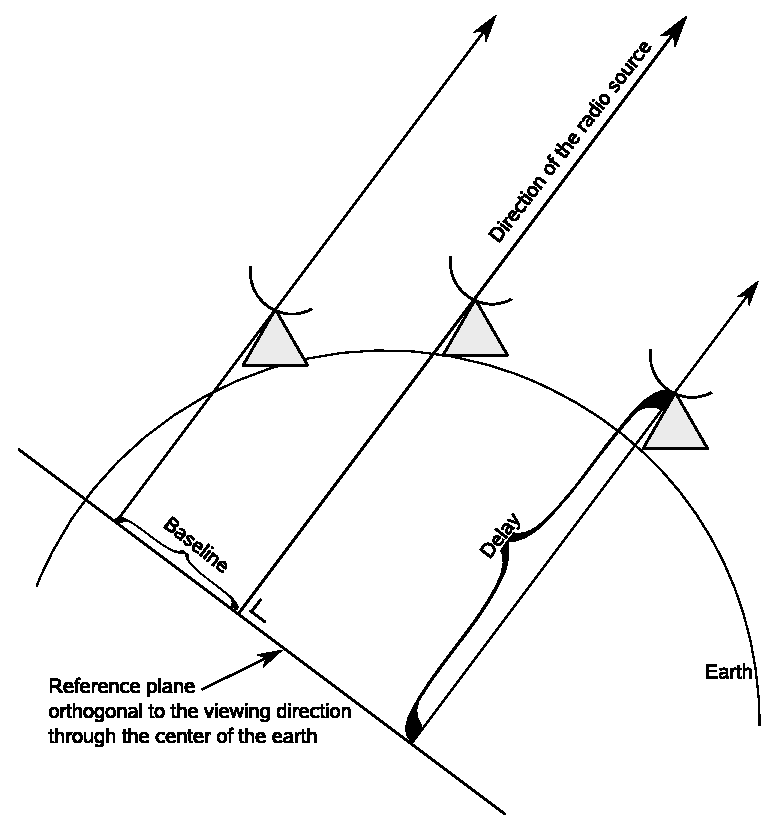
\includegraphics[width=.5\textwidth]
  {img/VLBI}
  \caption{Block diagram of the correlation.}
  \label{fig:correlation_diagram}
\end{figure}
\paragraph{Correlation}
Correlation is the process by which data from multiple telescopes is
collected and combined to measure the spatial Fourier components of
the image of the sky. The high data rates and the optimizations
complicate the process.

Assume that we are correlating the signal of two telescopes. First,
both signals are delayed to account for the different time at which
the signal arrives at the telescopes, see
Figure~\ref{fig:correlation_diagram}.  This process requires very
accurate timing information in the data and a very detailed model of
the geometry of the experiment. After the signals are properly
aligned, the signals are ready to be correlated. Correlation is a well
defined mathematical function~\cite{def_correlation} on two signals in
which the first signal is delayed with discrete steps and the integral
is computed of of the delayed signal multiplied with the second
signal. To increase the signal to noise ratio, the correlated signal
is averaged over a certain period of time. Typical averaging times lie
in the range of $0.25-4$ seconds.

For more than two stations, each station is correlated with itself
(auto-correlation) and every other station (cross-correlation). Note
that the complexity is quadratic in the number of telescopes.

\subsection{Platform}\label{sec:chap1}
The \das3\ supercomputer~\cite{das3} was deployed in the summer of
2007. It is distributed over 5 locations in the Netherlands and
connected by an photonic network called StarPlane. StarPlane is also a
research project funded by the Netherlands Organization for Scientific
Research (NWO) and carried out at two Dutch Universities: the
University of Amsterdam (UvA) and the Vrije Universiteit Amsterdam
(VU). The goals of the project is to build an
\textit{application-controlled photonic network}. 

In the e-Science community there is more and more reliance on
distributed collaborations where researchers cooperate remotely with
each other and use larger and larger datasets. In order to generalize
scientific utilization of world-size inter-connected grids, scientific
application have three major requirements:
\begin{itemize}
\item \emph{better performances}: an application is said performance
  limited if the resources needed to run it are not large enough to
  satisfy its needs. Performance limitations can have multiple
  origins: insufficient computing resources ormemory, high network
  latency or low network throughput.
  
\item \emph{isolated environment}: there are classes of applications
  that can only be executed if put in an isolated environment, where
  other users'application cannot interfere. Examples are real-time
  distributed application, or benchmarks that require reproducible
  result.

\item \emph{scheduling}: some application requires to be synchronized
  with "external events" (like having radio-telescope looking at a
  specific location in the sky at a specific date). In order to
  execute such application it is mandatory to schedule them and
  reserve the needed resource in advance.
\end{itemize}

The regular Internet best-effort Layer3 IP routing has great
flexibility but is slow and unpredictable; on the other hand,
dedicated \textit{lightpaths} as available in \textit{lambda
  Grids}~\cite{eslea-2007}, with their predictable delays and
throughputs offer good performances and guarantee on the Quality of
Service (QoS). StarPlane tries to fill the gap between the two
approaches by experiencing application-controlled dynamic photonic
network. The project's vision is that applications, having direct
control of the network paths, could make better use of the network
than if they were managed by a third party. Giving end user an access
to dedicated connection has been implemented in many of the current
research and education networks. The Dutch National Resarch and
Education network SURFnet is one of them. SURFnet6 deploys multiple
fiber optic rings that connect the academic and research locations
around The Netherlands. One of these rings connects the universities
in Leiden, Delft and Amsterdam, the locations of the \das3\ clusters.
Into this ring eight wavelengths constitute the StarPlane lightpaths.
The distinctive features of StarPlane in comparison with other similar
initiatives are the emphasis on fast reconfiguration times, in the
orders of seconds or sub-seconds, the use of photonic equipment in the
core, and the tigh coupling between the user application and the
offered networking service.

The rest of the paper is organized as follows. Section~\ref{sec:vlbi}
describes the architecture of the software correlator.
Section~\ref{sec:data_flow} describes the data flow within the
correlator and the use of StarPlane to optimize the efficiency. We
present benchmarks in Section~\ref{sec:benchmarks} and conclude the
paper with future work in Section~\ref{sec:conclusion}.

%%% Local Variables:
%%% mode: latex
%%% TeX-master: "Ingrid"
%%% End:
